\subsection{Puente LAN/GPIB para Windows E5810}

El E5810 actúa como un puente entre una red LAN y equipos que soporten conexión GPIB y/o RS-232.  Permite   realizar operaciones I/O para obtener mediciones de datos de manera local o remota desde la instrumentación GPIB o RS-232.

\begin{figure}[h!] 
	\centering
	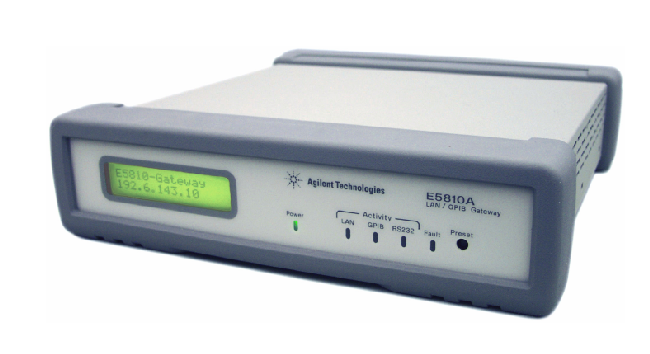
\includegraphics[width=10cm]{Imagenes/E5810.pdf}
	\caption{Puente LAN/GPIB Agilent E5810}
	\label{Fig:PuenteLanGPIB}
\end{figure}

\subsubsection{Interfaz de comunicaciones}
Conexiones de red

EL E5810 puede conectarse a una red de la dos siguientes formas: 

\begin{itemize}
	\item Conexión a una red empresarial.
	\item Conexión a una red local.
	\item Conexión directa a una PC.
\end{itemize}

El E5810 puede servir de puente para 14 instrumentos GPIB y para un (1) instrumento RS-232, vía red Ethernet  10BASE-T/100BASE-TX. El E5810 puede detectar la configuración de red y ajustarse de forma automática a la velocidad apropiada. Este equipo posee un conector RJ-45 en su parte posterior. 

\subsubsection{Software}

El E5810 incluye \emph{Agilent IO libraries Suite}, la cual incluye Agilent Virtual Instrument Software Architecture (VISA), VISA COM, Standard Control Library (SICL) y varias utilidades I/O. Este software provee compatibilidad con diferentes fabricantes de software y hardware. Provee una capa de software para operaciones I/O, permite utilizar varios lenguajes como Visual Basic, Visual C++ y Agilent VEE.
El E5810 soporta Dynamic Host Configuration Protocol (DCHP el cual le permite obtener su dirección de IP de forma automática. Por defecto el equipo puede usar DHCP, se puede deshabilitar DHCP y asignar una dirección estática IP al E5810.
El E5810 soporta todas operaciones I/O provistas por VISA, VISA COM, SICL y Agilent VEE. 
Como se muestra en la figura 1, el PC posee las aplicaciones cliente VISA LAN, TCP/IP LAN, necesarias para acceder al E5810. El E5810 posee un servidor LAN además de firmware TCP/IP LAN que le permite actuar como un servidor LAN.
El software cliente realiza conexión con el servidor remoto dentro del E5810, establecida la conexión, el cliente envía peticiones I/O al servidor E5810 a través de la red al servidor E5810, el software instalado en la PC cliente VISA LAN emplea la suite de protocolos TCP/IP LAN para ello. El servidor del E5810 ejecuta estas peticiones de I/O en el instrumento GPIB o RS-232 apropiado.
El E5810 pude servir a múltiples clientes conectados en un momento dado. La cantidad máxima de clientes concurrentes depende del uso de memoria de E5810, la cual esta determinada por el numero de clientes y el numero de sesiones que corren estos clientes. Existe un máximo de 16 clientes accediendo de forma concurrente.
Múltiples instrumentos GPIB se pueden conectar al bus GPIB, pero solo una operación de I/O puede ocurrir en el bus GPIB en un momento dado. Solo se ejecuta una petición de un cliente a la vez, las demás deben esperar hasta que el cliente actual termine. El primer cliente en acceder es el primer cliente servido (cola FIFO).
En caso de que el cliente requiera realizar una secuencia de operaciones I/O que no deban ser interrumpidas, el cliente debe obtener un lock sobre la interfaz GPIB del dispositivo. Completada la operación debe liberar el lock.





